\section{Un QCM}

Pour chacune des questions ci-dessous, une seule des quatre réponses est proposées est exacte. On demande d'indiquer cette réponse. Aucune justification n'est demandée.

\begin{questions}
	\question[] Au premier trimestre, un élève a obtenu les notes suivantes en mathématiques : 9 ; 9 ; 11 ; 14 ; 17
	
	\begin{parts}
		\part[] L'étendue est :
		\begin{oneparcheckboxes}
			\choice 4
			\correctchoice 8
			\choice 9
			\choice 10
		\end{oneparcheckboxes}
	
		\part[] La moyenne est :
		\begin{oneparcheckboxes}
			\choice 11
			\correctchoice 12
			\choice 13
			\choice 14
		\end{oneparcheckboxes}
	
		\part[] La médiane est :
		\begin{oneparcheckboxes}
			\choice 10
			\choice \num{10.5}
			\correctchoice 11
			\choice \num{11.5}
		\end{oneparcheckboxes}
	\end{parts}


	\question[] On considère le diagramme en boite ci-dessous :
	
	\begin{center}
		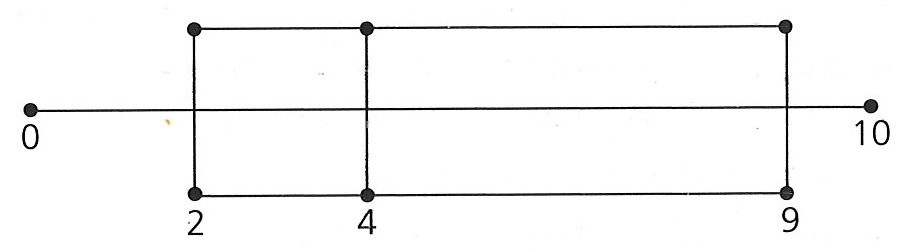
\includegraphics[scale=1]{moustache}
	\end{center}
	
	\begin{checkboxes}
		\correctchoice la médiane est 4 ;
		\choice le troisième quartile est 10 ;
		\choice l'intervalle interquartile est $[0; 10]$ ;
		\choice le premier quartile est 4.
	\end{checkboxes}
	
\end{questions}